\documentclass[__main__.tex]{subfiles}

\begin{document}
\paragraph{Э-16}
Движущийся со скоростью $\vec v$ электрон, попадает в однородные и взаимно перпендикулярные электрическое $\vec E$ и магнитное $\vec B$ поля. Скорость электрона перпендикулярна обоим полям. Найдите траекторию движения электрона.\\

Мы решаем нерелятивистский случай. А значит $\nu \ll 1$.\\
$\vec B || \vec (OZ)$ и $\vec E || \vec (OY)$.\\
Тогда уравнения движения будут иметь вид:
$$
m\dot{\vec\nu} = e\vec E+e\vec\nu\times\vec B,
$$
Или, в нашем случае:
\begin{gather*}
\begin{cases}
m\ddot x= e\dot y B \\
m\ddot y = eE_y-e\dot x B=eE-e\dot x B \\
m\ddot z = eE_z=0
\end{cases},
\end{gather*}

\begin{wrapfigure}[34]{r}{0.3\linewidth}
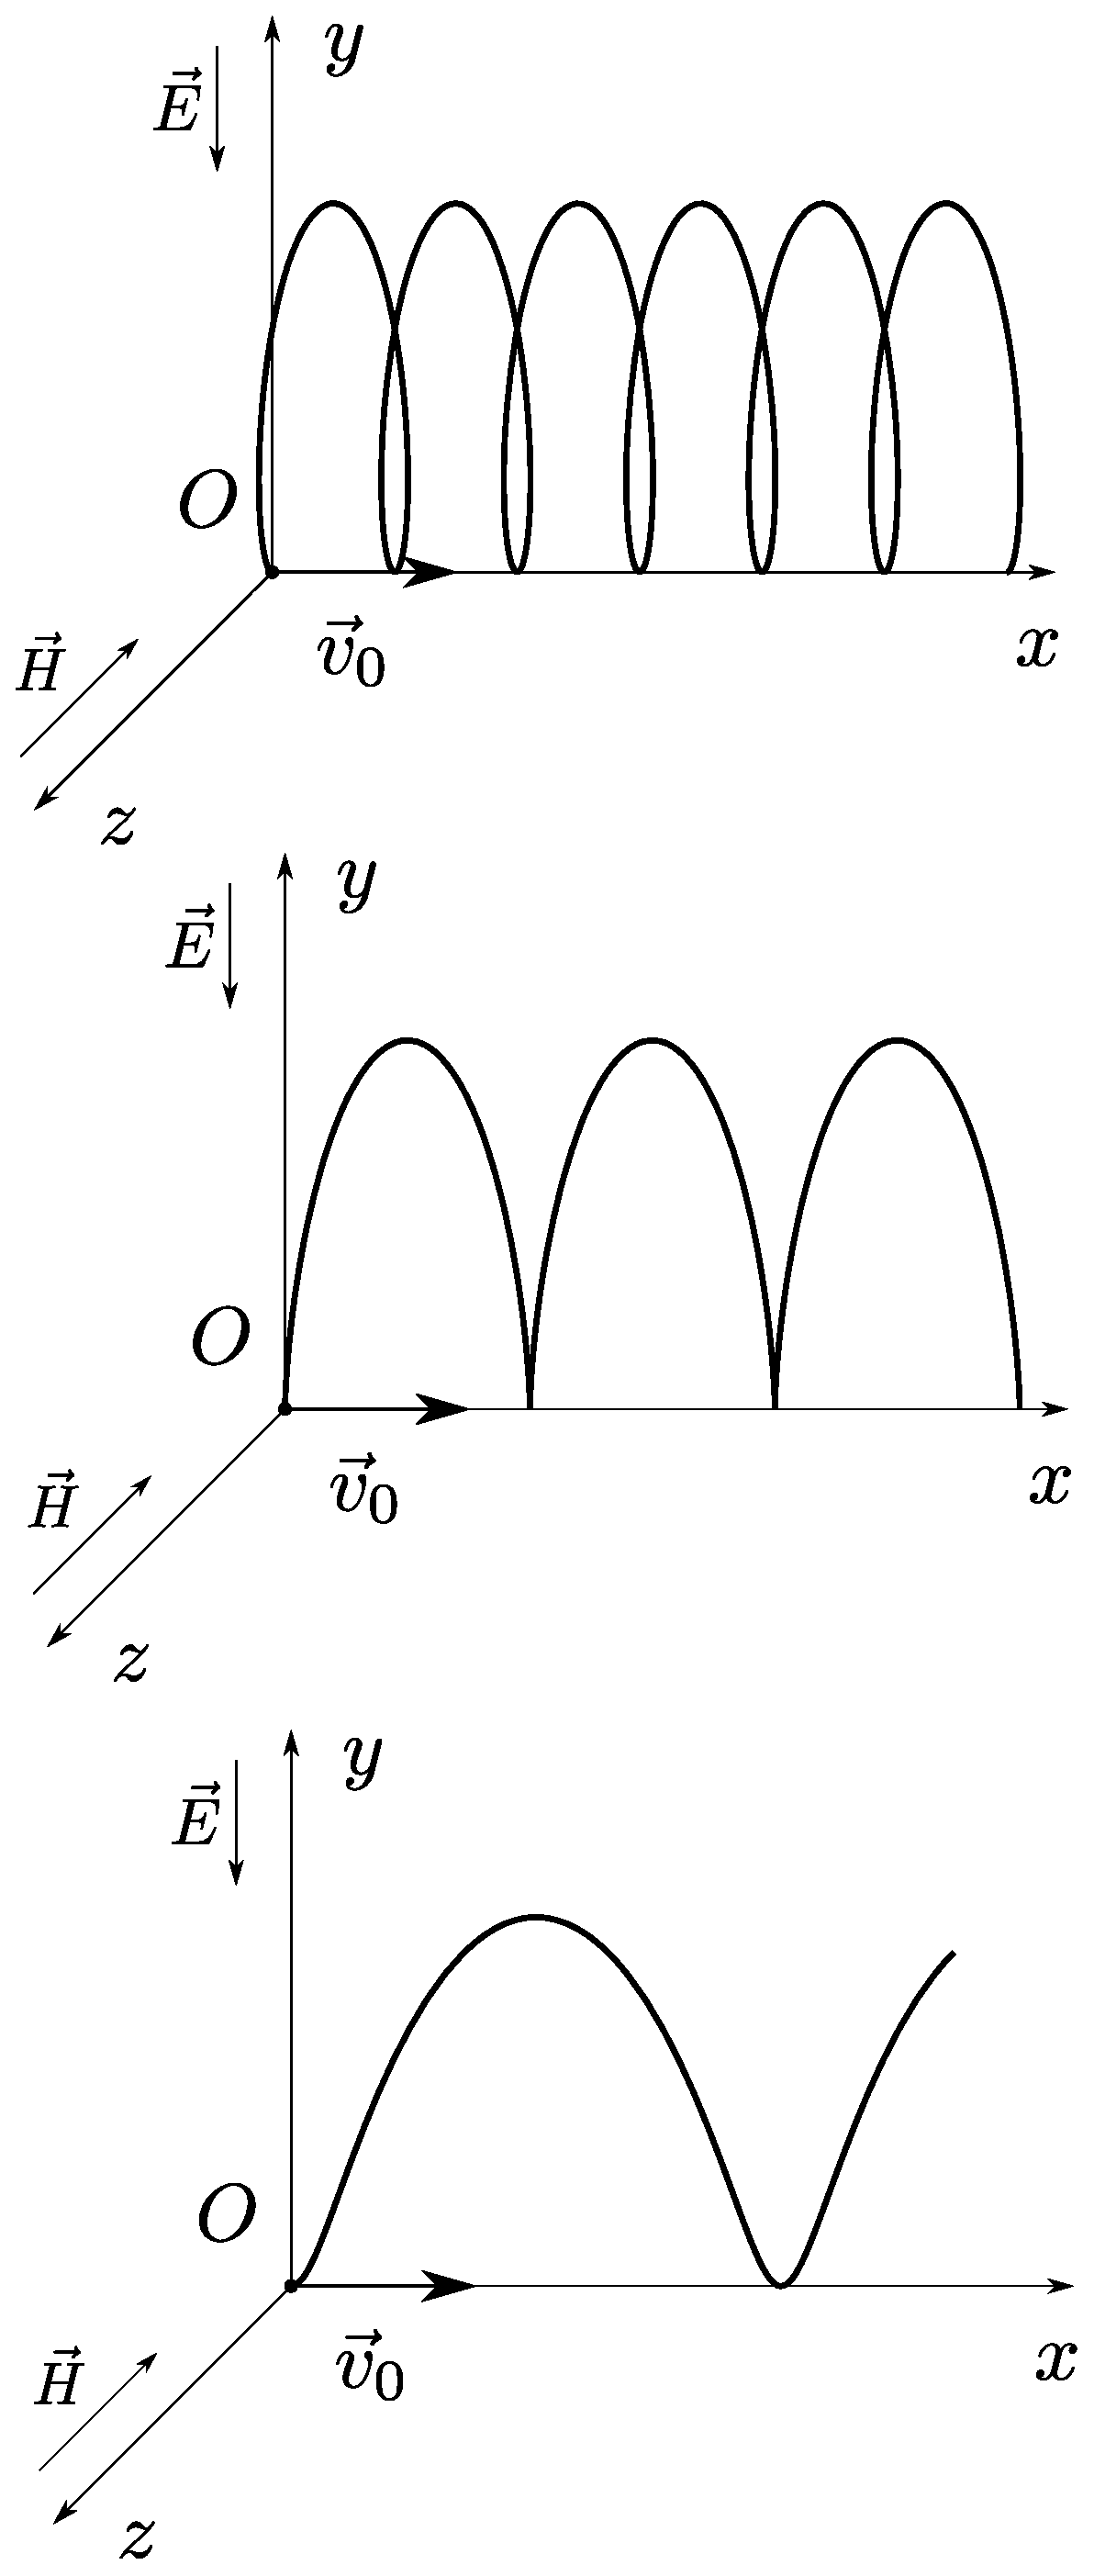
\includegraphics[width=1\linewidth]{e-16}
\caption{Качественно различные траектории частицы.}
\end{wrapfigure}

Умножим второе уравнение (для $\ddot y$) на $i$ и сложим с первым, положив $\dot z = \dot x + i \dot y$:
$$
\frac{d}{dt}\dot z+i\omega\dot z = i\frac{e}{m}E
$$
Где $\omega = \frac{eB}{m}$. Решение этого дифференциального уравнения примет вид:
$$
\dot x + i\dot y=\alpha e ^{-i\omega t}+\frac{E}{B}
$$

В общем случае $\alpha$ - комплексное число, однако правильно выбрав начало отсчета времени мы можем сделать так, что умножение на $e^{-i\omega t}$ избавит нас от хлопот, и, как следствие, сделает $\alpha$ действительным.\\

Отделяя комплексные переменные от действительных получим пару уравнений:
\begin{flalign*}
\begin{split}
\dot x &= \alpha \cos(\omega t)+ \frac{E}{B} \\
\dot y &= -\alpha \sin(\omega t)
\end{split},
\end{flalign*}

Очевидно , что
\begin{flalign*}
\begin{split}
x &= \frac{\alpha}{\omega} \sin(\omega t)+ \frac{Et}{B}\\
y &= \frac{\alpha}{\omega} \cos(\omega t)-1
\end{split}
\end{flalign*}

Пределы интегрирования выставлялись так, что $x(0)=y(0)=0$.\\
Собственно, в зависимости от соотношения параметров параметрических уравнений возможно три качественно различных случая, которые и изображены на рисунках.
\end{document}